%%!TEX encoding = UTF-8 Unicode

% Several lines in file have comments suggesting common packages for the
% typical thesis in informatics or electronics developed at UA
% uncomment/comment the lines as required for your work
% Before each optional line you will have a small comment

% According to UA rules, font size should range from 10 to 12pt.
\documentclass[11pt,a4paper,oneside,onecolumn]{memoir}

\listfiles

\usepackage[utf8]{inputenc}

% Select Computer Modern Typewritter (For bold ttfamily in listings)
\usepackage{lmodern}
% OR... Bera Mono
%\usepackage[scaled]{beramono} % TTT Font
%\usepackage{anyfontsize} % As the name says...

\usepackage[T1]{fontenc}

% Enable for for Overleaf support
\usepackage{ifthen}
\def\useoverleaf{0}  % change to non-zero (for instance, 1) to enable it

\makeatletter
\newcommand{\makecoverfile}[0]{%
  \immediate\write18{latexmk -pdf cover.tex}%
}
\makeatother

\usepackage{tcolorbox}


% For PDF merging
\usepackage{pdfpages}

% Set DPI to 300
\pdfpxdimen=\dimexpr 1in/300\relax

% Allow the use of a larger number of packages
\usepackage{morewrites} 

% For English and Portuguese languages
% Portuguese will be the default.
% Uncomment \setlanguage below to change it
\usepackage[english,portuguese]{babel}

% Uncomment to use a custom date format
%\usepackage{datetime}
%\newdateformat{thesisdate}{\monthname[\THEMONTH] \THEYEAR} % Month Year

% Make pdf look better
\usepackage{microtype} 

% Uncomment to enable floats on facing pages
%\usepackage{dpfloat}

% Side by side figures
% Eg. Fig 1a, Fig 1b
\usepackage[hang,small,bf]{caption}
%\let\tion\undefined
%\let\subfloat\undefined
\usepackage{subcaption}

%\RequirePackage{textcase}

% Dropped Caps
%\usepackage{lettrine}

% Configure Hyperlink color
% As a matter or style, you may use this to enable/disable color boxes on links
%\usepackage[breaklinks=true,colorlinks=false,linkcolor=blue]{hyperref}
% Or use the default values provided by the hyperref package
\usepackage{hyperref}

% Redefine section names according to your preference
%\def\sectionautorefname{Section}
%\def\chapterautorefname{Chapter}
%\def\figureautorefname{Figure}
%\def\listingautorefname{Listing}
%\def\tableautorefname{Table}

% Redefine code boxes
\ifthenelse{\equal{\useoverleaf}{0}}
{\usepackage{minted}}

\addto\captionsportuguese{%
  \renewcommand\listingscaption{Código}
}
\fvset{fontsize=\footnotesize} % Make Code blocks smaller than text
\usepackage{csquotes}

% Add support for PDF Comments
\usepackage{comment}
\ifthenelse{\equal{\useoverleaf}{0}}
{\usepackage{pdfcomment}}{}
\usepackage{bookmark} % New Bookmarks

% For Multiple columns in Glossary
\usepackage{multicol}

% Add support for Math symbols
\usepackage{amsmath}
\usepackage{amssymb}

% Add support for graphics
\usepackage{graphicx}

% Add support for Colors
\usepackage{xcolor}

% Add support for the Euro symbol
\usepackage{eurosym}

% Add support for missingfigure and todo
\usepackage{todonotes}

% Setup bibliography with Biber using IEEE style for proper UTF-8 support
\usepackage[backend=biber, style=ieee, sorting=none, natbib=true, mincitenames=1, maxcitenames=2]{biblatex}
\bibliography{bib/references.bib}

% Use acronyms
\usepackage[printonlyused]{acronym} % For acronyms

% Indenting the first paragraph after section start
\usepackage{indentfirst}

% For fixing listoflistings with memoir
\usepackage{xparse}

% Uncomment the next lines to enable chart support through pgf and tikz
% This may require you to install further packages in your Tex system
%\usepackage[version=0.96]{pgf}
%\usepackage{tikz}

% UML support
%\usepackage{pgf-umlsd}

% Trees, Arrows, Mindmaps and other popular objects
%\usetikzlibrary{arrows,shadows,trees,shapes,decorations,automata,backgrounds,petri,mindmap} % for pgf-umlsd

% Package to master SI units
\usepackage[detect-weight=true]{siunitx}
% For Electric Circuits
%\sisetup{load-configurations = binary}

% Set Voltage direction accordingly
% Option : oldvoltagedirection,nooldvoltagedirection,RPvoltages,EFvoltages
% More information at: https://mirrors.ibiblio.org/CTAN/graphics/pgf/contrib/circuitikz/doc/circuitikzmanual.pdf
% By default this template is using the Old Voltage Direction
%\usepackage[oldvoltagedirection,american,cuteinductors,smartlabels]{circuitikz}
%\usetikzlibrary{calc}
%\ctikzset{bipoles/thickness=1}
%\ctikzset{bipoles/length=0.8cm}
%\ctikzset{bipoles/diode/height=.375}
%\ctikzset{bipoles/diode/width=.3}
%\ctikzset{tripoles/thyristor/height=.8}
%\ctikzset{tripoles/thyristor/width=1}
%\ctikzset{bipoles/vsourceam/height/.initial=.7}
%\ctikzset{bipoles/vsourceam/width/.initial=.7}
%\tikzstyle{every node}=[font=\small]
%\tikzstyle{every path}=[line width=0.8pt,line cap=round,line join=round]

% For inline TT text (e.g. code snippets)
\usepackage{verbatim}

% Frames around figures and allow force placement
\usepackage{float}

% Configure Float style
%\floatstyle{boxed}
%\restylefloat{table}
%\restylefloat{figure}
%\restylefloat{lstlisting}

% For test purposes you may use the lipsum package to create dummy text
\usepackage{lipsum} % REMOVE

%Keep floats inside section!
\usepackage[section]{placeins}
\let \oldsubsubsection \subsubsection
\renewcommand{\subsubsection}[2][]{
  \FloatBarrier
  \oldsubsubsection#1{#2}
}
\let \oldsubsection \subsection
\renewcommand{\subsection}[2][]{
  \FloatBarrier
  \oldsubsection#1{#2}
}
\let \oldsection \section
\renewcommand{\section}[2][]{
  \FloatBarrier
  \oldsection#1{#2}
}
\let \oldchapter \chapter
\renewcommand{\chapter}[2][]{
  \FloatBarrier
  \oldchapter#1{#2}
}



% Use the built-in division styling
\headstyles{memman}

% Include subsections in the TOC
\settocdepth{subsection}

% Numbering down to subsections as well
\setsecnumdepth{subsection}

% extra index for first lines
\makeindex[lines]

% Margins for University of Aveiro Thesis
\setlrmarginsandblock{3cm}{2.5cm}{*}
\setulmarginsandblock{3cm}{3cm}{*}
\checkandfixthelayout

% Or select your custom spacing to make any ajustment
%\addtolength{\parskip}{0.5\baselineskip}
\linespread{1.5}

\newcommand\mainmatterWithoutReset
{\edef\temppagenumber{\arabic{page}}%
  \mainmatter
  \setcounter{page}{\temppagenumber}%
}


%%%%%%%%%%%%%%%%%%%%%%%%%%%%%%%%%%%%%%%%%%%%%%%%%%
% Document begins here
%%%%%%%%%%%%%%%%%%%%%%%%%%%%%%%%%%%%%%%%%%%%%%%%%%

\begin{document}

% Fix the numbering scheme by having a ghost style for page numbering
\pagenumbering{Alph}

\ifthenelse{\equal{\useoverleaf}{0}}{}{\makecoverfile{}}%
\setcounter{page}{0}\includepdf[pages=-]{cover.pdf}

% Uncomment to enable English
%\selectlanguage{english}


% Front matter

%Custom Chapter style named `thesis`
\makechapterstyle{thesis}{% Based on ell
  \chapterstyle{default}
  \renewcommand*{\chapnumfont}{\normalfont\sffamily}
  \renewcommand*{\chaptitlefont}{\normalfont\Huge\sffamily}
  \settowidth{\chapindent}{\chapnumfont 111}
  \renewcommand*{\chapterheadstart}{\begingroup
    \vspace*{\beforechapskip}%
    \begin{adjustwidth}{}{-\chapindent}%
    \hrulefill
    \smash{\rule{0.4pt}{15mm}}
    \end{adjustwidth}\endgroup}
  \renewcommand*{\printchaptername}{}
  \renewcommand*{\chapternamenum}{}
  \renewcommand*{\printchapternum}{%
    \begin{adjustwidth}{}{-\chapindent}
    \hfill
    \raisebox{10mm}[0pt][0pt]{\fontsize{30}{25}\selectfont\chapnumfont \thechapter}%
                              \hspace*{1em}
    \end{adjustwidth}\vspace*{-3.0\onelineskip}}
  \renewcommand*{\printchaptertitle}[1]{%
    \vskip\onelineskip
    \raggedleft {\chaptitlefont ##1}\par\nobreak\vskip 4\onelineskip}}


% Select chapter style from existing or select custom
%\chapterstyle{thesis} % Others: dowding, demo2, dash, chappell, brotherton, bianchi, ger, madsen, tatcher, veelo,indexes)
% thesis can also be used as defined previously
% Check the memoir documentation for the available themes
% Default is veelo
\chapterstyle{veelo}
\makeoddfoot{plain}{}{\thepage}{} % Added by André Zúquete to fix a page numbering issue on the veelo chapter style

% Select Page style
\pagestyle{plain}

% If you feel adventurous you can also define all aspects of your theme
% Use either this input or the chapterstyle before
% % Rules
\newcommand{\thinRule}{\rule{\textwidth}{0.25pt}}

% Customize heading appearances
% Define styles
\newcommand{\partSize}{\Huge}
\newcommand{\partStyle}{\lsstyle\scshape}
\newcommand{\chapterSize}{\Huge}
\newcommand{\chapterStyle}{\lsstyle\scshape}
\newcommand{\chapterAfter}{}
\newcommand{\sectionSize}{\Large}
\newcommand{\sectionStyle}{\scshape\MakeTextLowercase}
\newcommand{\subsectionSize}{\large}
\newcommand{\subsectionStyle}{\scshape\MakeTextLowercase}
\newcommand{\subsubsectionSize}{\large}
\newcommand{\subsubsectionStyle}{\scshape\MakeTextLowercase}
\newlength{\partNumSizePt}
\setlength{\partNumSizePt}{60pt}
\newlength{\chapterNumSizePt}
\setlength{\chapterNumSizePt}{60pt}
\newcommand{\partNumSize}{%
  \fontsize{\partNumSizePt}{1.2\partNumSizePt}\selectfont%
}
\newcommand{\partNumStyle}{\partChapterNumColor}
\newcommand{\chapterNumSize}{%
  \fontsize{\chapterNumSizePt}{1.2\chapterNumSizePt}\selectfont%
}
\newcommand{\chapterNumStyle}{\partChapterNumColor}

% Customize parts
\renewcommand{\partnamefont}{\partSize\partStyle}
\renewcommand{\partnumfont}{\partNumSize\partNumStyle}
\renewcommand{\printpartname}{}
\renewcommand{\printparttitle}[1]{%
  \normalfont\normalcolor\partnamefont #1
}

% Customize chapters
\makeatletter
\setlength{\beforechapskip}{30pt}
\renewcommand*{\chapterheadstart}{\vspace*{\beforechapskip}}
\setlength{\afterchapskip}{3ex}
\setlength{\midchapskip}{3ex}
\renewcommand*{\chapnamefont}{%
  \Large\flushright\chapterStyle\partChapterNumColor%
}
\renewcommand*{\chapnumfont}{\chapterNumSize\chapterNumStyle}
\renewcommand*{\chaptitlefont}{%
  \normalfont\flushleft\normalcolor\chapterSize\chapterStyle%
}
\renewcommand*{\printchaptername}{%
  \chapnamefont\MakeTextLowercase{\@chapapp}%
}
\renewcommand*{\chapternamenum}{\quad}
\renewcommand*{\printchapternum}{%
%  \chapnumfont\textls[-75]{\classicstylenums{\thechapter}}%
 \chapnumfont\textls[-75]{\thechapter}%

}
\renewcommand*{\printchaptertitle}[1]{%
  \chaptitlefont #1
  \chapterAfter
}
\makeatother
% Customize sections and subsections
\setsecnumformat{\csname my#1\endcsname\quad}
\setsecheadstyle{\sectionSize\sectionStyle}
\newcommand{\mysection}{{\thesection}}
\setlength{\beforesecskip}{3em}


\setsubsecheadstyle{\subsectionSize\subsectionStyle}
\newcommand{\mysubsection}{{\normalfont\subsectionSize\thesubsection}}
\setlength{\beforesubsecskip}{3em}

\setsubsubsecheadstyle{\subsubsectionSize\subsubsectionStyle}
\newcommand{\mysubsubsection}{{\normalfont\subsubsectionSize\thesubsubsection}}
\setlength{\beforesubsubsecskip}{2em}

% Customize "Table of ..." appearance
% Customize headings
\newcommand{\renewPrintXTitle}[1]{%
  \renewcommand{#1}[1]{%
    \printchaptertitle{##1}%
  }%
}
\renewPrintXTitle{\printtoctitle}
\renewPrintXTitle{\printlottitle}
\renewPrintXTitle{\printloftitle}

% Customize ToC headings
\renewcommand{\cftpartfont}{\partChapterNumColor\partStyle}
\renewcommand{\cftchapterfont}{\chapterStyle}
\renewcommand{\cftsectionfont}{}
\renewcommand{\cftsubsectionfont}{}
\renewcommand{\cftfigurefont}{}
\renewcommand{\cfttablefont}{}
\newcommand{\cftlstlistingfont}{}

% Increase number width
\newlength{\cftNumWidthIncrease}
\setlength{\cftNumWidthIncrease}{0.25em}
\addtolength{\cftpartnumwidth}{\cftNumWidthIncrease}
\addtolength{\cftchapternumwidth}{\cftNumWidthIncrease}
\addtolength{\cftsectionindent}{\cftNumWidthIncrease}
\addtolength{\cftsubsectionindent}{\cftNumWidthIncrease}
% No leader dots
%\renewcommand*{\cftpartdotsep}{\cftnodots}
%\renewcommand*{\cftchapterdotsep}{\cftnodots}
%\renewcommand*{\cftsectiondotsep}{\cftnodots}
%\renewcommand*{\cftsubsectiondotsep}{\cftnodots}
%\renewcommand*{\cftfiguredotsep}{\cftnodots}
%\renewcommand*{\cfttabledotsep}{\cftnodots}
%\newcommand*{\cftlstlistingdotsep}{\cftnodots}
% Set page numbers immediately after entry text
\newcommand{\tocEntryPageSep}{\hspace{1em}}
\renewcommand{\cftpartleader}{\cftdotfill{\cftdotsep}}
%\renewcommand{\cftpartafterpnum}{\cftparfillskip}
%\renewcommand{\cftchapterleader}{\tocEntryPageSep}
\renewcommand{\cftchapterleader}{\cftdotfill{\cftdotsep}}
%\renewcommand{\cftchapterafterpnum}{\cftparfillskip}
\renewcommand{\cftsectionleader}{\cftdotfill{\cftdotsep}}
%\renewcommand{\cftsectionafterpnum}{\cftparfillskip}
\renewcommand{\cftsubsectionleader}{\cftdotfill{\cftdotsep}}
%\renewcommand{\cftsubsectionafterpnum}{\cftparfillskip}
\renewcommand{\cftfigureleader}{\cftdotfill{\cftdotsep}}
%\renewcommand{\cftfigureafterpnum}{\cftparfillskip}
\renewcommand{\cfttableleader}{\cftdotfill{\cftdotsep}}
%\renewcommand{\cfttableafterpnum}{\cftparfillskip}
\newcommand{\cftlstlistingleader}{\cftdotfill{\cftdotsep}}
%\newcommand{\cftlstlistingafterpnum}{\cftparfillskip}
% Customize page numbers
\newcommand{\tocPageStyle}{\tocPageColor}
\renewcommand{\cftpartpagefont}{\tocPageStyle}
\renewcommand{\cftchapterpagefont}{\tocPageStyle}
\renewcommand{\cftsectionpagefont}{\tocPageStyle}
\renewcommand{\cftsubsectionpagefont}{\tocPageStyle}
\renewcommand{\cftfigurepagefont}{\tocPageStyle}
\renewcommand{\cfttablepagefont}{\tocPageStyle}
\newcommand{\cftlstlistingpagefont}{\tocPageStyle}

% Abstract
% Remove indents around abstract text
\setlength{\absleftindent}{0pt}
\setlength{\absrightindent}{0pt}
% Change font size to conform with the rest of the document text
\renewcommand{\abstracttextfont}{\normalsize}

% Customize headers and footers including page numbers
\newcommand{\hfTextSize}{\footnotesize}
\newcommand{\headTextStyle}{\lsstyle\scshape\MakeTextLowercase}
\nouppercaseheads
\makeevenhead{headings}%
             {\hfTextSize\thepage}%
             {}%
             {\hfTextSize\headTextStyle\leftmark}
\makeevenhead{plain}%
             {\hfTextSize\thepage}%
             {}%
             {\hfTextSize\headTextStyle\leftmark}
\makeoddhead{headings}%
            {\hfTextSize\headTextStyle\rightmark}%
            {}%
            {\hfTextSize\thepage}
\makeoddhead{plain}%
            {\hfTextSize\headTextStyle\rightmark}%
            {}%
            {\hfTextSize\thepage}


% Customize captions
\newcommand{\captionSize}{\small}
\newcommand{\captionStyle}{\scshape}
\newcommand{\captionWidthRatio}{0.9}

\captionnamefont{\captionSize\captionStyle}
\captiontitlefont{\captionSize}
\captiondelim{ -- }
\captiontitlefinal{}
\changecaptionwidth
%\captionwidth{\captionWidthRatio\textwidth}

% Define colors
%\newcommand{\titleColor}{\color[rgb]{0.616, 0.0627, 0.176}}
\newcommand{\titleColor}{\color[rgb]{0,0,0}}

\newcommand{\partChapterNumColor}{\titleColor}
\newcommand{\dropCapColor}{\titleColor}
%\newcommand{\tocPageColor}{\color[rgb]{0.0980, 0.329, 0.651}}

\newcommand{\tocPageColor}{\color[rgb]{0, 0,0}}
\definecolor{shade0}{rgb}{1.0 , 1.0 , 1.0 }
\definecolor{shade1}{rgb}{0.9 , 0.9 , 0.9 }
\definecolor{shade2}{rgb}{0.8 , 0.8 , 0.8 }
\definecolor{shade3}{rgb}{0.65, 0.65, 0.65}
\definecolor{shade4}{rgb}{0.45, 0.45, 0.45}
\definecolor{shade5}{rgb}{0.0 , 0.0 , 0.0 }



%Exclude sub figures from List of Figures
%\captionsetup[subfloat]{list=no}

% Texts
\newenvironment{introduction}
{%
  \begin{minipage}{\textwidth}%
   \itshape%
}
{%
  \end{minipage}%
  \par\addvspace{2\baselineskip plus 0.2\baselineskip minus 0.2\baselineskip}%
}

\frontmatter

\tightlists
\midsloppy
\raggedbottom

\setcounter{tocdepth}{2} %subsections are added to the TOC
\setcounter{secnumdepth}{4} %subsubsections are numbered

% Initial document tables start here: TOC, LOF, LOT, Glossary
% Table of contents with slightly smaller font
{\small\tableofcontents}

% List of figures with slightly smaller font
\clearpage
{\small\listoffigures}

% List of tables with slightly smaller font
\clearpage
{\small\listoftables}

% List of code snippets

% Fix for Listings with memoir

\RenewDocumentCommand \chapter { s O{#3} m }{%
  \FloatBarrier
  \IfValueTF{#1}  % if optional star is seen
    {\oldchapter*{#2}}
    {\oldchapter#1{#2}}
}

%\renewcommand{\listingscaption}{Código}
%\renewcommand{\listoflistingscaption}{Lista de Excertos de Código}
%\clearpage
%{\small\listoflistings}
%\addcontentsline{toc}{chapter}{\listoflistingscaption}

% Reset Chapters
\renewcommand{\chapter}[2][]{
  \FloatBarrier
  \oldchapter#1{#2}
}

% Print Glossary
\clearpage
\small
\chapter{Glossário}

\footnotesize
\SingleSpacing

\begin{multicols}{2}
\begin{acronym}[AAAAAA]

	\acro{ML}[ML]{Machine Learning}
	\acro{DL}[DL]{Deep Learning}
	\acro{AI}[AI]{Artificial Intelligence}
	\acro{NLP}[NLP]{Natural Language Processing}
	\acro{APWG}[APWG]{Anti-Phishing Working Group}
	\acro{RFC}[RFC]{Request for Comments}
	\acro{IC3}[IC3]{Internet Crime Complaint Center}
	\acro{FBI}[FBI]{Federal Bureau of Investigation}
	\acro{SVM}[SVM]{Support Vector Machine}
	\acro{CNN}[CNN]{Convolutional Neural Network}
	\acro{RNN}[RNN]{Recurrent Neural Network}
	\acro{LSTM}[LSTM]{Long Short-Term Memory}
	\acro{TF-IDF}[TF-IDF]{Term Frequency-Inverse Document Frequency}
	\acro{BERT}[BERT]{Bidirectional Encoder Representations from Transformers}
	\acro{DistilBERT}[DistilBERT]{Distilled Bidirectional Encoder Representations from Transformers}
	\acro{RoBERTa}[RoBERTa]{A Robustly Optimized BERT Pretraining Approach}
	\acro{SPF}[SPF]{Sender Policy Framework}
	\acro{DKIM}[DKIM]{DomainKeys Identified Mail}
	\acro{DMARC}[DMARC]{Domain-based Message Authentication, Reporting, and Conformance}
	\acro{MTA-STS}[MTA-STS]{Mail Transfer Agent Strict Transport Security}
	\acro{TLS}[TLS]{Transport Layer Security}

\end{acronym}
\end{multicols}


\normalsize

%%%%%%%%%%%%%%%%%%%%%%%%%%%%%%%%%%%%%%%%%%%%%%%%%%%%%%%
% Main document starts here
%%%%%%%%%%%%%%%%%%%%%%%%%%%%%%%%%%%%%%%%%%%%%%%%%%%%%%%

\mainmatter

% Line spacing: 1.5 pt 
\OnehalfSpacing

%%%%%%%%%%%%%%%%%%%%%%%%%%%%%%%%%%%%%%%%%%%%%%%%%%%%%%%
% Start of Thesis text 
%%%%%%%%%%%%%%%%%%%%%%%%%%%%%%%%%%%%%%%%%%%%%%%%%%%%%%%

% Uncomment to add further chapters
\chapter{Introdução}%
\label{chapter:introduction}

\begin{introduction}
A short description of the chapter.

A memorable quote can also be used.
\end{introduction}



\section{Acrónimos}

Primeira e seguintes referências: \ac{h2o}, \ac{h2o}

Plural, acrónimo expandido e curto: \acp{h2o}, \acl{h2o}, \acs{h2o}

Com citação\footnote{Necessária entrada na bibliografia}: \ac{adsl}, \ac{adsl}


\section{Fontes}

\begin{itemize}
\item{\tiny Tiny}
\item{\scriptsize Scriptsize}
\item{\footnotesize Footnotes}
\item{\small Small}
\item{\normalsize Normal}
\item{\large large}
\item{\Large Large}
\item{\LARGE LARGE}
\item{\huge huge}
\item{\Huge Huge}
\end{itemize}

\section{Unidades}

Utilizando o pacote \verb|siunitx| é possível utilizar unidades do Sistema Internacional. Exemplo: a aceleração da gravidade é de \SI{9.8}{\metre\per\second\squared} e um ficheiro ocupa \SI{1}{\mebi\byte}. 

\section{Code Blocks}
%\lipsum[5]
Uma listagem pode ser apresentada com o ambiente \texttt{listing}, que é um float (objeto flutuante, tal como uma figura ou uma tabela).

A listagem em Código~\ref{lbl:snippet-test} mostra um exemplo em C.

\begin{listing}[h]
\begin{minted}{c}

#include <stdio.h>
#define N 10
/* Block
 * comment */
 
int main()
{
    int i;
 
    // Line comment.
    puts("Hello world!");
 
    for (i = 0; i < N; i++)
    {
        puts("LaTeX is also great for programmers!");
    }
 
    return 0;
}
\end{minted}
\caption{This caption appears below the code.}
\label{lbl:snippet-test}
\end{listing}

%\lipsum[5]

\section{Citações}

Algumas formas distintas de citar:

\begin{itemize}
    \item \textbf{Apenas referência}:~\cite{rfc44}
    \item \textbf{Apenas data}:~\citedate{rfc44}
    \item \textbf{Apenas ano}:~\citeyear{rfc44}
    \item \textbf{Apenas autor}:~\citeauthor{rfc44}
    \item \textbf{Apenas editor}:\citelist{rfc44}{organization}
    \item \textbf{Autor e referência}:\citet{rfc44}
\end{itemize}

\chapter{State of the Art}

This chapter presents the state of the art that will set the stage for the work developed in this dissertation.

\section{E-mail and .eml}

E-mail, short for electronic mail, is a method of exchanging messages over the internet or computer networks. It is one of the most widely used forms of digital communication today, with billions of users worldwide. E-mail remains a central medium not only for legitimate communication but also as a primary attack vector exploited by cybercriminals through phishing and malware distribution.

From a technical perspective, e-mail is structured according to the Internet Message Format (\acs{RFC} 5322), which defines the standard headers and body content of a message, such as sender, recipient, subject, date, and message body \cite{rfc5322}. This specification was later updated by \acs{RFC} 6854, which introduced support for group syntax in the From: and Sender: header fields, thereby allowing messages to represent multiple authors or senders in a structured and standardized manner \cite{rfc6854}. Individual messages can be stored and exchanged as .eml files, a format that encapsulates the full message including metadata (headers), body text, and attachments using the MIME standard. The .eml format is particularly relevant in research contexts, as it preserves raw information such as authentication results, routing paths, and content features that are useful for forensic analysis and machine learning-based detection approaches.

As one of the most popular communication tools, e-mail has become a prime target for cyber attacks. Its widespread use, combined with the inherent trust users place in messages that appear legitimate, makes e-mail an ideal vector for malicious actors seeking to steal sensitive information, distribute malware, or manipulate recipients into performing certain actions. Among the various threats that exploit e-mail, phishing has emerged as one of the most prevalent and damaging, leveraging social engineering techniques to deceive users into revealing credentials, financial information, or other confidential data.

\section{Phishing}

Phishing is a type of cyber attack in which an attacker attempts to deceive individuals into providing sensitive information, such as usernames, passwords, or financial details, by disguising as a trustworthy entity through electronic communication channels, most commonly e-mail. Phishing attacks often employ social engineering tactics, exploiting users’ trust, fear, or curiosity, and can include malicious links, fraudulent websites, or deceptive attachments.

In 2024, according to the \ac{APWG}, phishing attacks have been on a decline, totaling 3.7 million attacks, down roughly 24\% from 2023.

\begin{figure}[ht]
    \centering
    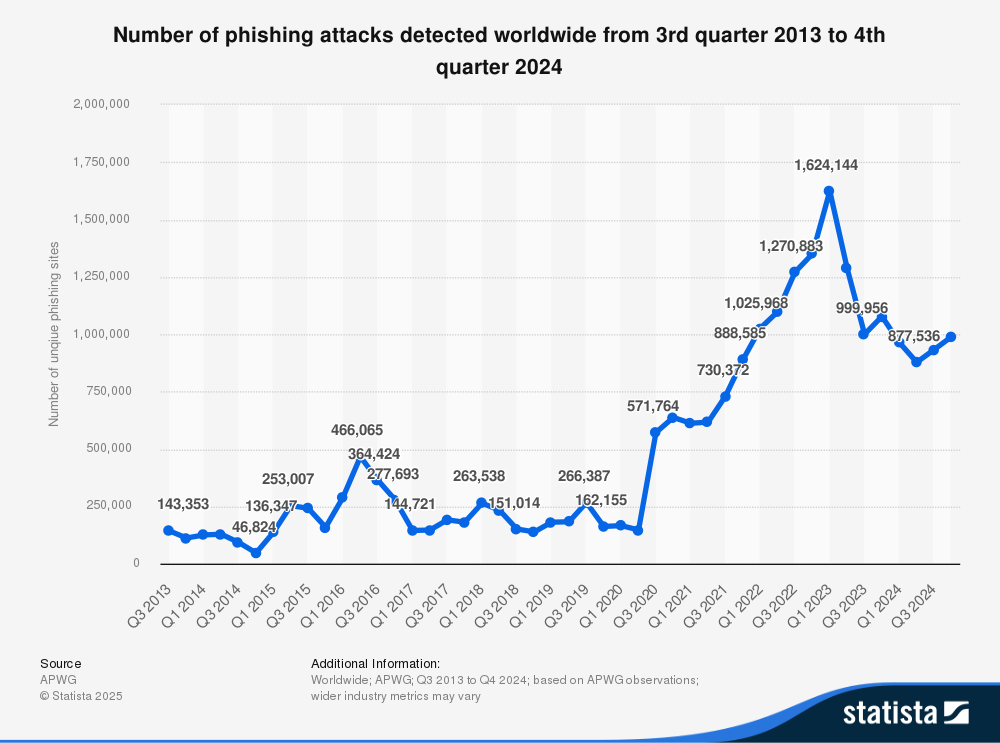
\includegraphics[width=0.8\textwidth]{figs/phishing_trends.png}
    \caption{Number of Phishing Attacks over time (Source: APWG)}
    \label{fig:phishing_trends}
\end{figure}

Although a decrease in attacks is a positive sign, phishing remains a significant threat due to its adaptability and the increasing sophistication of attacks. According to the \acs{IC3} 2024 \acs{FBI} report, phishing attacks resulted in the loss of USD 70 million, clearly showing that phishing is still a relevant threat \cite{IC32024}. These attacks often coincide with larger data breaches, further magnifying their impact on organizations and individuals.

To mitigate the threat of phishing, a wide range of technical solutions has been developed. 
These include email authentication protocols such as \ac{SPF}, \ac{DKIM}, and \ac{DMARC}, which help verify the legitimacy of senders and reduce the likelihood of spoofed messages reaching users’ inboxes \cite{DEROUET20165}.

Transport-layer protections like \ac{MTA-STS} and \ac{TLS} reporting further strengthen the security of email delivery, ensuring that messages are transmitted securely between servers and are less vulnerable to interception or tampering.

Additionally, advanced \ac{ML} and \ac{DL} approaches have been increasingly applied to detect phishing attempts. Models can leverage features extracted from email headers, body content, URLs, and attachments, with recent transformer-based architectures and embedding techniques providing state-of-the-art performance in identifying both traditional and sophisticated phishing messages.

\section{Machine Learning and Deep Learning for Phishing Detection}

\ac{ML} and \ac{DL} approaches have been the subject of extensive research in the context of phishing detection.
Attackers have been using \ac{AI} to create more convincing phishing emails, and as such, researchers are increasingly focusing on developing robust detection mechanisms that can adapt to evolving threats.

Traditional machine learning techniques are no longer sufficient to combat the sophisticated nature of modern phishing attacks \cite{Fernandes2024}. Most systems relied heavily on engineered features extracted from emails, including header fields (such as sender or received chain), lexical and textual cues (e.g., \ac{TF-IDF} and bag-of-words), URL tokenization, structural HTML features, and attachment metadata. These features were typically fed into classical classifiers, such as \ac{SVM}, Random Forests, Naive Bayes, or Logistic Regression. Early deep learning models, including \acp{CNN} and \acp{RNN}/\ac{LSTM}, were also applied to textual and structural components, providing promising results but still often being outperformed by well-engineered classical approaches. 

Since then, there have been several significant advances in the \ac{ML}/\ac{DL} space for email-based phishing detection:

Pretrained transformer architectures, like \ac{BERT}, \ac{DistilBERT}, and \ac{RoBERTa}, have been fine-tuned for phishing detection tasks. These models effectively encode the email body, subject lines, and sometimes HTML structure into embeddings that capture semantic and contextual signals beyond simple lexical overlaps \cite{uddin2025}.

Modern systems more often integrate multiple input modalities: authentication metadata (\ac{SPF}/\ac{DKIM}/\ac{DMARC}), header features, embedding representations of textual content, URL encoders, HTML structure features, and outputs from attachment analysis or sandbox environments \cite{PATRA2025110403, electronics12204261}.

Another technique used to detect phishing is vector similarity search. This technique involves converting raw emails into high-dimensional vectors using transformer embeddings. These vectors can then be compared to identify similarities between emails, using methods such as cosine similarity or Euclidean distance. Although this approach yielded better results than traditional \ac{ML} techniques, it was still outperformed by fine-tuned transformer models \cite{PATRA2025110403}.

\section{Sentiment Analysis}

While most research focuses on technical and structural features of phishing emails, a section of analysis that has been largely overlooked is sentiment analysis.

Sentiment analysis involves using \ac{NLP} techniques to identify and extract subjective information from text, such as emotions, opinions, or attitudes. In the context of phishing detection, sentiment analysis can provide insights into the emotional tone and persuasive strategies employed by attackers. This can help cyber security professionals better understand the psychological tactics used, and possibly protect email users from said entity of being targeted by certain tactics, like blackmail.

In previous works, sentiment or tone was occasionally used as one auxiliary signal: existing works might include keyword frequency (urgency / fear words), lexical heuristics (e.g. counts of exclamation marks, imperative mood etc.). However, these were generally simpler, lexicon-based or manually curated features.

Most models prioritized content / URL / header / attachment features, leaving sentiment / emotional tone as a minor axis of research. This, combined with the fact that in many datasets, the emotional manipulation was implicit rather than explicitly annotated, meant that sentiment features were often noisy or under-utilized.

In a recent work, \ac{DistilBERT} was used to extract embeddings that carry sentiment / tone information, that was fed into a classical \ac{SVM}. This was compared to simply using \ac{SVM} by itself, and the results showed that the sentiment-aware model outperformed the baseline by a 3\% margin in F1-score (97\% vs 94\%) \cite{salian2024enhancing}.

Another work, "Comparative Investigation of Traditional Machine-Learning Models and Transformer Models for Phishing Email Detection", explicitly stated that results could be further improved by "incorporating sentiment analysis techniques to detect social-engineering tactics and to better understand the emotional tone and intent behind the email content" \cite{electronics13244877}.

As such, its clear that a well annotated dataset with sentiment labels, not just positive / negative labels, could provide valuable insights into the emotional manipulation tactics used in phishing emails, and potentially improve detection performance.


\chapter{Dataset Creation and Annotation}

As presented by the previous chapter, the performance of machine learning models is highly dependent on the quality and quantity of the training data. In this chapter, we describe the process of creating and annotating the dataset used for training and evaluating our model.

\section{Dataset Creation}

Since for this study we only required a dataset of the email body content labeled for its emotions, we created our own dataset by taking the existing dataset used in \cite{Fernandes2024} and feeding it into a \ac{LLM} to generate a larger dataset. 

The dataset used required no preprocessing, as it was already in a clean, well-structured format tailored for our needs. The dataset consisted of approximately 480 samples of email body content, each labeled with one of fourteen possible emotions.

To create our dataset, we took all emails related to a certain emotion and prompted the Ollama \ac{LLM} to generate additional samples by providing context and examples, using the following prompt template:

\begin{tcolorbox}[colback=gray!10, colframe=gray!60, title={Prompt Template}]
Based on these examples of emails expressing '{emotion}', generate 1 new realistic phishing email that captures the same emotional tone and style. Make it convincing and professional, evoking the emotion of {emotion}.

Generate only the email content, no additional text or explanations: \textit{Example emails here}
\end{tcolorbox}


Using this method, we were able to create a new dataset with 10,000 samples, equatily distributed across the fourteen emotions. This expanded dataset provided a robust foundation for training our machine learning models to accurately classify the emotional content of phishing emails.

Below is an example of a generated email for the emotion "Admiration":

\begin{tcolorbox}[colback=gray!5, colframe=gray!40, title={Example Email — Admiration}]
\obeylines
\textbf{Subject:} A surprise awaits you — Unlock your exclusive benefits today!

Dear [Recipient],

We hope this message finds you well and thriving! We're thrilled to inform you that our records indicate an outstanding opportunity for you — one that we believe will bring joy and appreciation to your day.

Over the years, you've been a valued member of our community. Your dedication, passion, and unwavering commitment have not gone unnoticed. In recognition of your remarkable journey with us, we're delighted to offer you a special surprise — an exclusive upgrade on your current subscription plan with our esteemed organization.

This gesture is but a small token of admiration for your contributions and the positive impact you've made. We trust this unexpected delight will bring a smile to your face and serve as a reminder that your efforts are truly valued.

To unveil the details of your special benefits, please click on the following link: [suspicious link]

Warmest regards,
[Your Name]
[Your Position/Title]
[Organization Name]
\end{tcolorbox}

\section{Annotation Guidelines}

To ensure consistency and accuracy in the annotation process, we established a set of guidelines for annotators to follow. 

\section{Dataset Annotation}

With the dataset created, and guidelines set, we proceeded to annotate the dataset. Given that the dataset was generated using a \ac{LLM} with specific prompts, each sample was inherently labeled with the intended emotion. However, to ensure the quality and accuracy of these labels, we conducted a manual review process.

Since it's infeasible to annotate all 10,000 samples with just one annotator, and to eliminate potential biases, we decided on using a annotation plataform called Doccano \cite{doccano} hosted on a DigitalOcean \ac{VM} \cite{digitalocean}. This platform allows multiple annotators to work on the same dataset, providing a collaborative environment for annotation.

%\include{chapter4}

%%%%%%%%%%%%%%%%%%%%%%%%%%%%%%%%%%%%%%%%%%%%%%%%%%%%%%%
% End of Thesis text 
%%%%%%%%%%%%%%%%%%%%%%%%%%%%%%%%%%%%%%%%%%%%%%%%%%%%%%%

\backmatter

%%%%%%%%%%%%%%%%%%%%%%%%%%%%%%%%%%%%%%%%%%%%%%%%%%%%%%%
% Print all used references
%%%%%%%%%%%%%%%%%%%%%%%%%%%%%%%%%%%%%%%%%%%%%%%%%%%%%%%

\begingroup
\renewcommand{\bibfont}{\footnotesize}
% Redefine References name to Portuguese
% Change if you are using english
\defbibheading{bibliography}[References]{
	\chapter{#1}
}
\SingleSpacing
\setlength\bibitemsep{8pt}
\printbibliography[heading=bibliography]
\endgroup


%%%%%%%%%%%%%%%%%%%%%%%%%%%%%%%%%%%%%%%%%%%%%%%%%%%%%%%
% Load appendix
%%%%%%%%%%%%%%%%%%%%%%%%%%%%%%%%%%%%%%%%%%%%%%%%%%%%%%%

\mainmatterWithoutReset
\appendix

\chapter{Additional content}


\end{document}
